\subsection{基于MVC框架的数据库应用开发}

\begin{frame}[allowframebreaks,fragile]{什么是MVC}
\begin{columns}
\begin{column}{0.4\textwidth}
\begin{itemize}
    \item MVC框架包含三个部分每个部分各自处理自己的工作,互不干扰
    \begin{itemize}
        \item 业务模型控制器 (Controller)
        \item 业务模型 (Model)
        \item 用户结果呈现 (View)
    \end{itemize}
\end{itemize}
\end{column}

\begin{column}{0.6\textwidth}
\begin{figure}
    \centering
    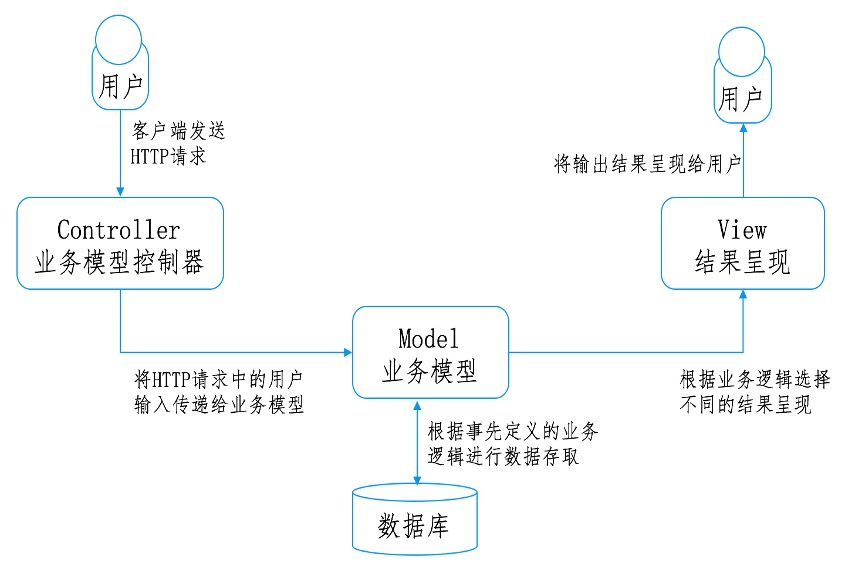
\includegraphics[width=\textwidth]{figure/fig-15.jpg}
\end{figure}
\end{column}

\end{columns}
\end{frame}


\begin{frame}[allowframebreaks,fragile]{什么是MVC}
\begin{columns}
\begin{column}{0.4\textwidth}
\begin{itemize}
    \item \textcolor{red}{业务模型控制器}:接收用户通过浏览器发送的HTTP服务请求
    \begin{itemize}
        \item 包括用户需要选择的业务模型,以及其它可选的输入参数
        \item 可以是用户在文本框中输入的文本、下拉列表框中的数据项等
        \item 也可以是用户的操作类型
    \end{itemize}
\end{itemize}
\end{column}

\begin{column}{0.6\textwidth}
\begin{figure}
    \centering
    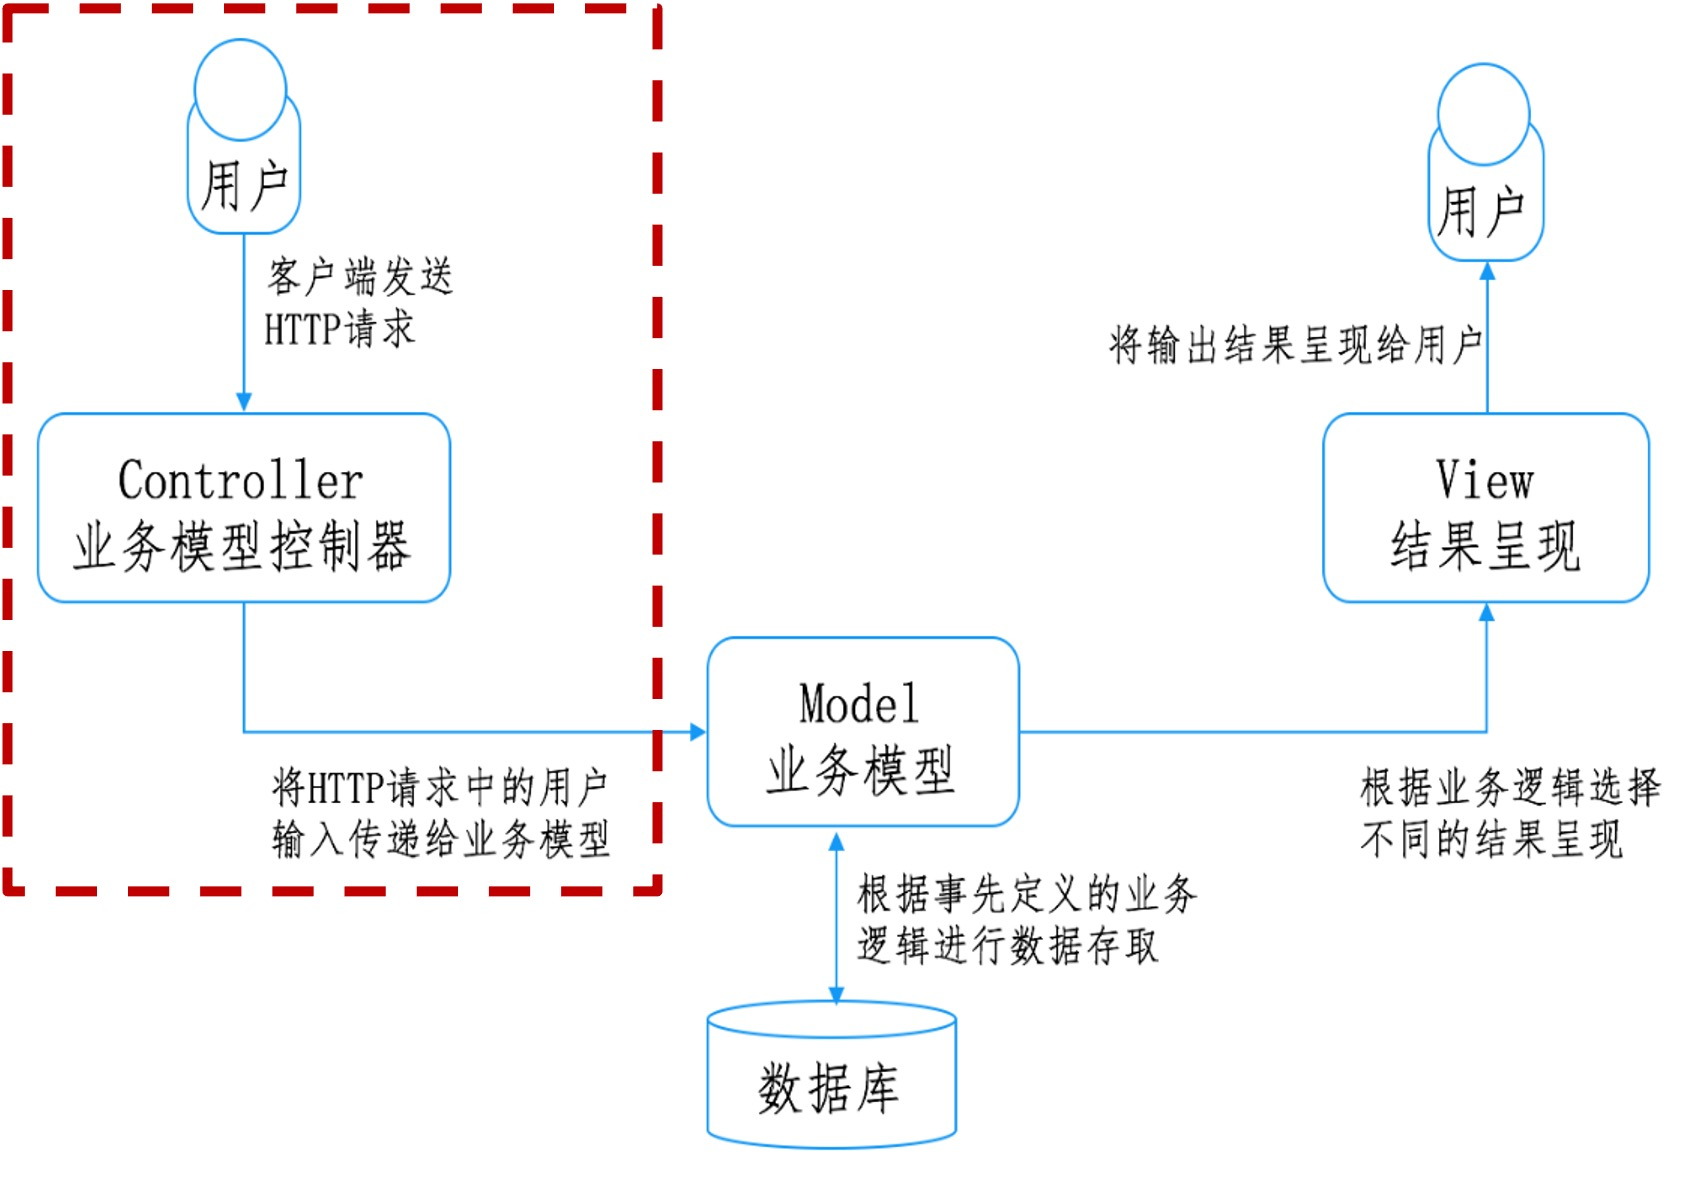
\includegraphics[width=\textwidth]{figure/fig-16.jpg}
\end{figure}
\end{column}

\end{columns}
\end{frame}


\begin{frame}[allowframebreaks,fragile]{什么是MVC}
\begin{columns}
\begin{column}{0.4\textwidth}
\begin{itemize}
    \item \textcolor{red}{业务模型}:建立用户的业务逻辑
    \begin{itemize}
        \item 解析出来的用户数据,执行事先定义的业务逻辑,并操纵数据库存取数据
        \item 输出独立于具体的数据格式,可为多个用户结果呈现提供展示所需要的数据,减少了代码的重复性
    \end{itemize}
\end{itemize}
\end{column}

\begin{column}{0.6\textwidth}
\begin{figure}
    \centering
    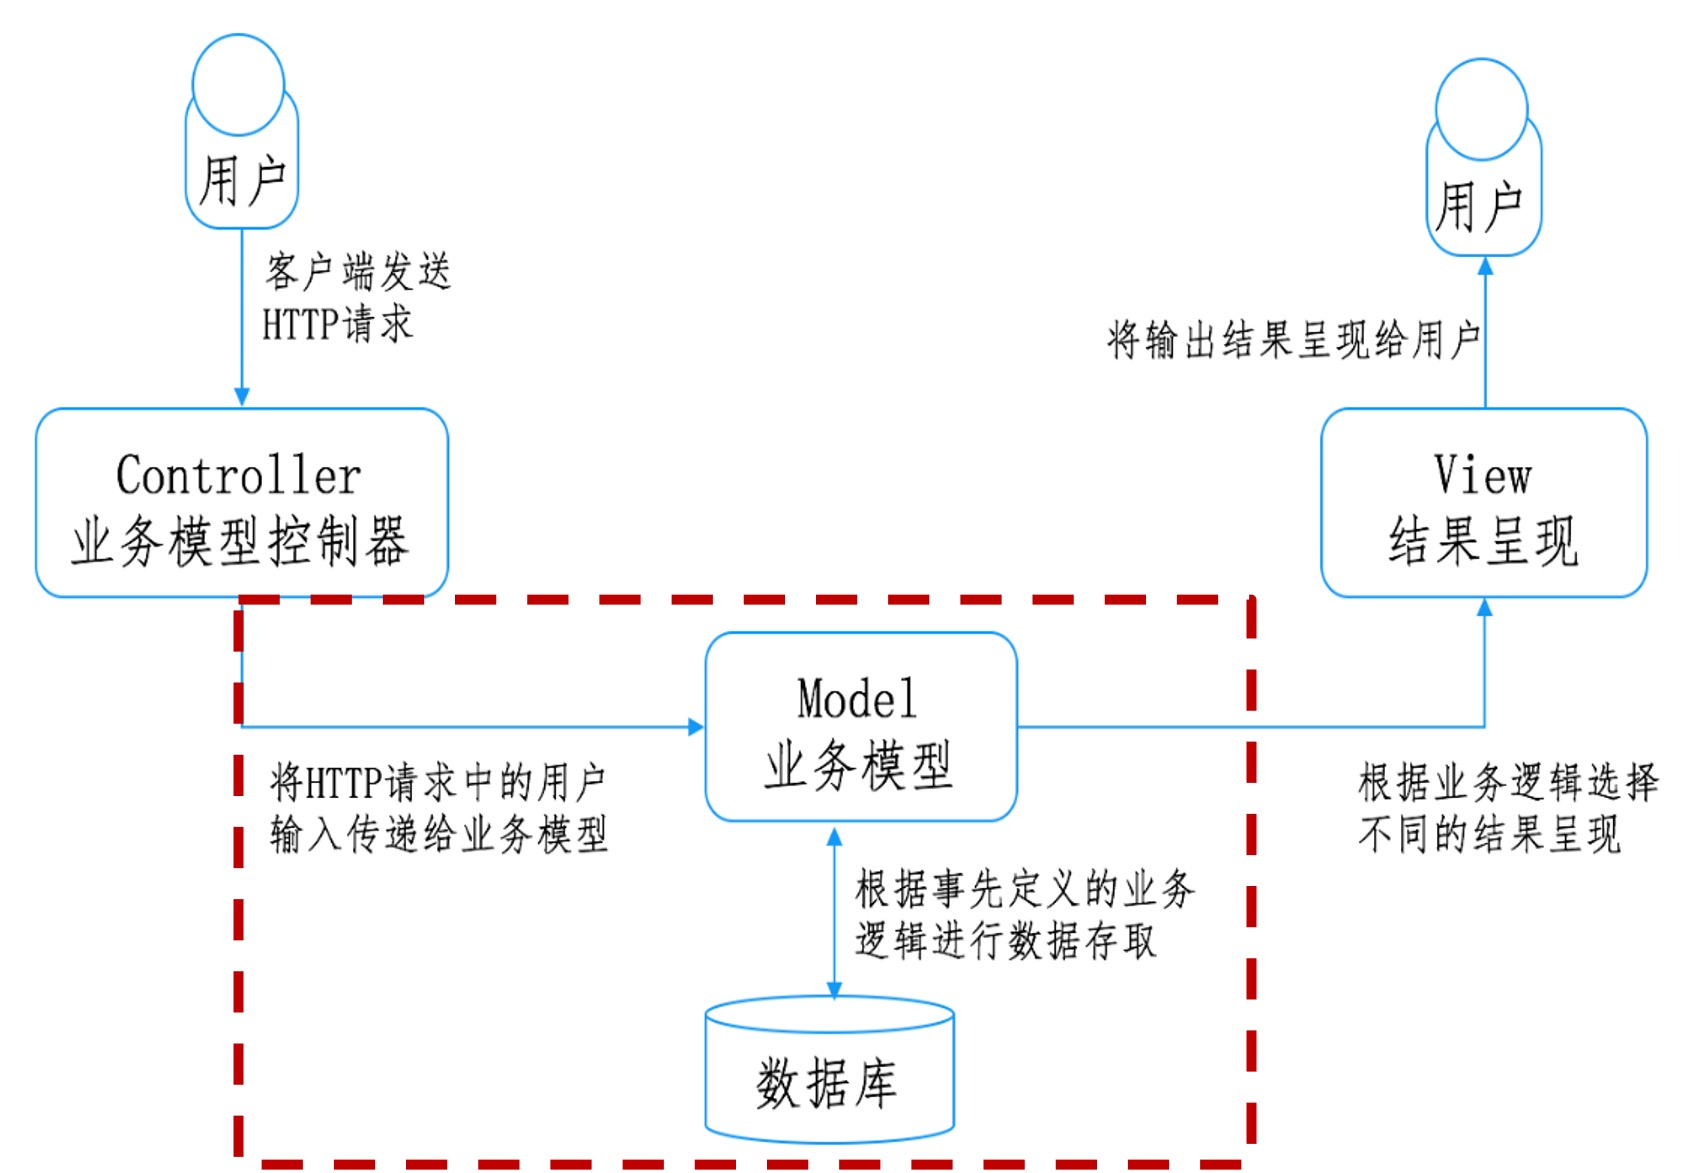
\includegraphics[width=\textwidth]{figure/fig-17.jpg}
\end{figure}
\end{column}

\end{columns}
\end{frame}


\begin{frame}[allowframebreaks,fragile]{什么是MVC}
\begin{columns}
\begin{column}{0.4\textwidth}
\begin{itemize}
    \item \textcolor{red}{用户结果呈现}:用户看到并与之交互获得结果展示的界面
    \begin{itemize}
        \item 根据业务模型输出的结果反馈给客户端进行呈现
    \end{itemize}
\end{itemize}
\end{column}

\begin{column}{0.6\textwidth}
\begin{figure}
    \centering
    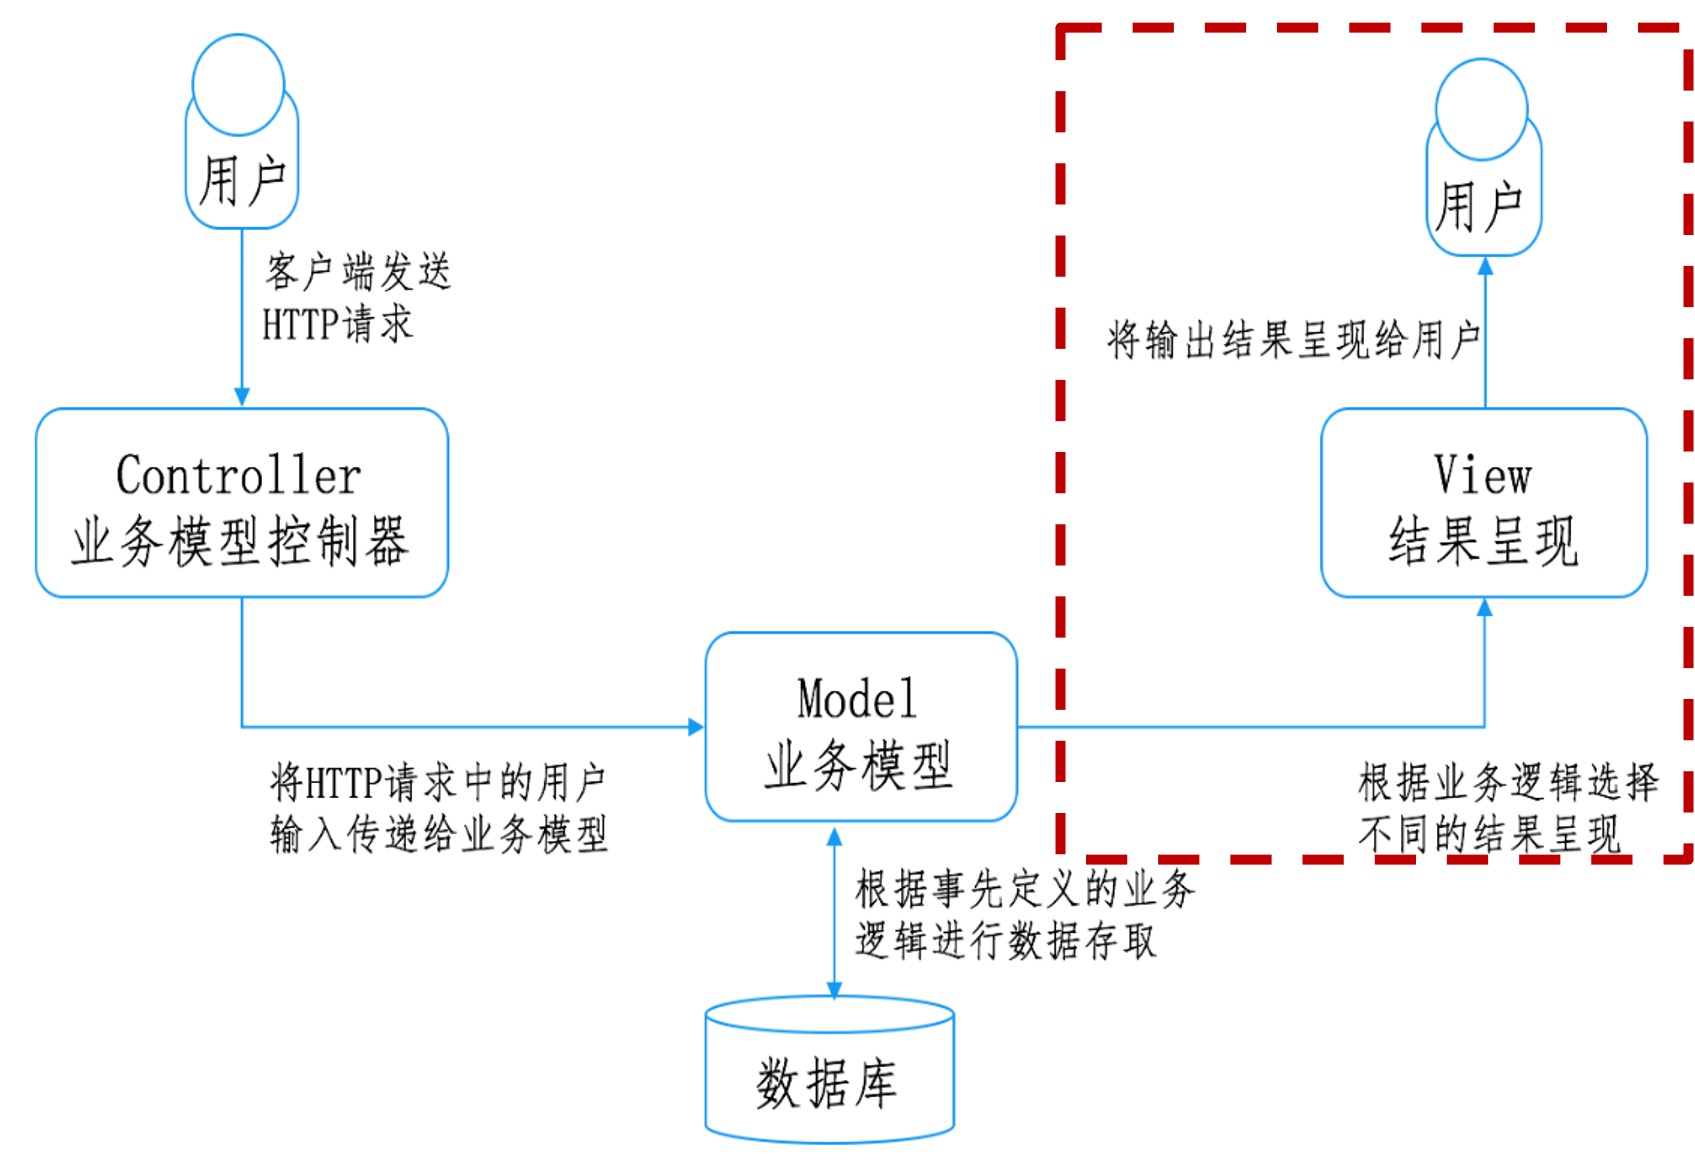
\includegraphics[width=\textwidth]{figure/fig-18.jpg}
\end{figure}
\end{column}

\end{columns}
\end{frame}



\begin{frame}[allowframebreaks,fragile]{使用MVC框架实现任务4的系统流程图}
\begin{figure}
    \centering
    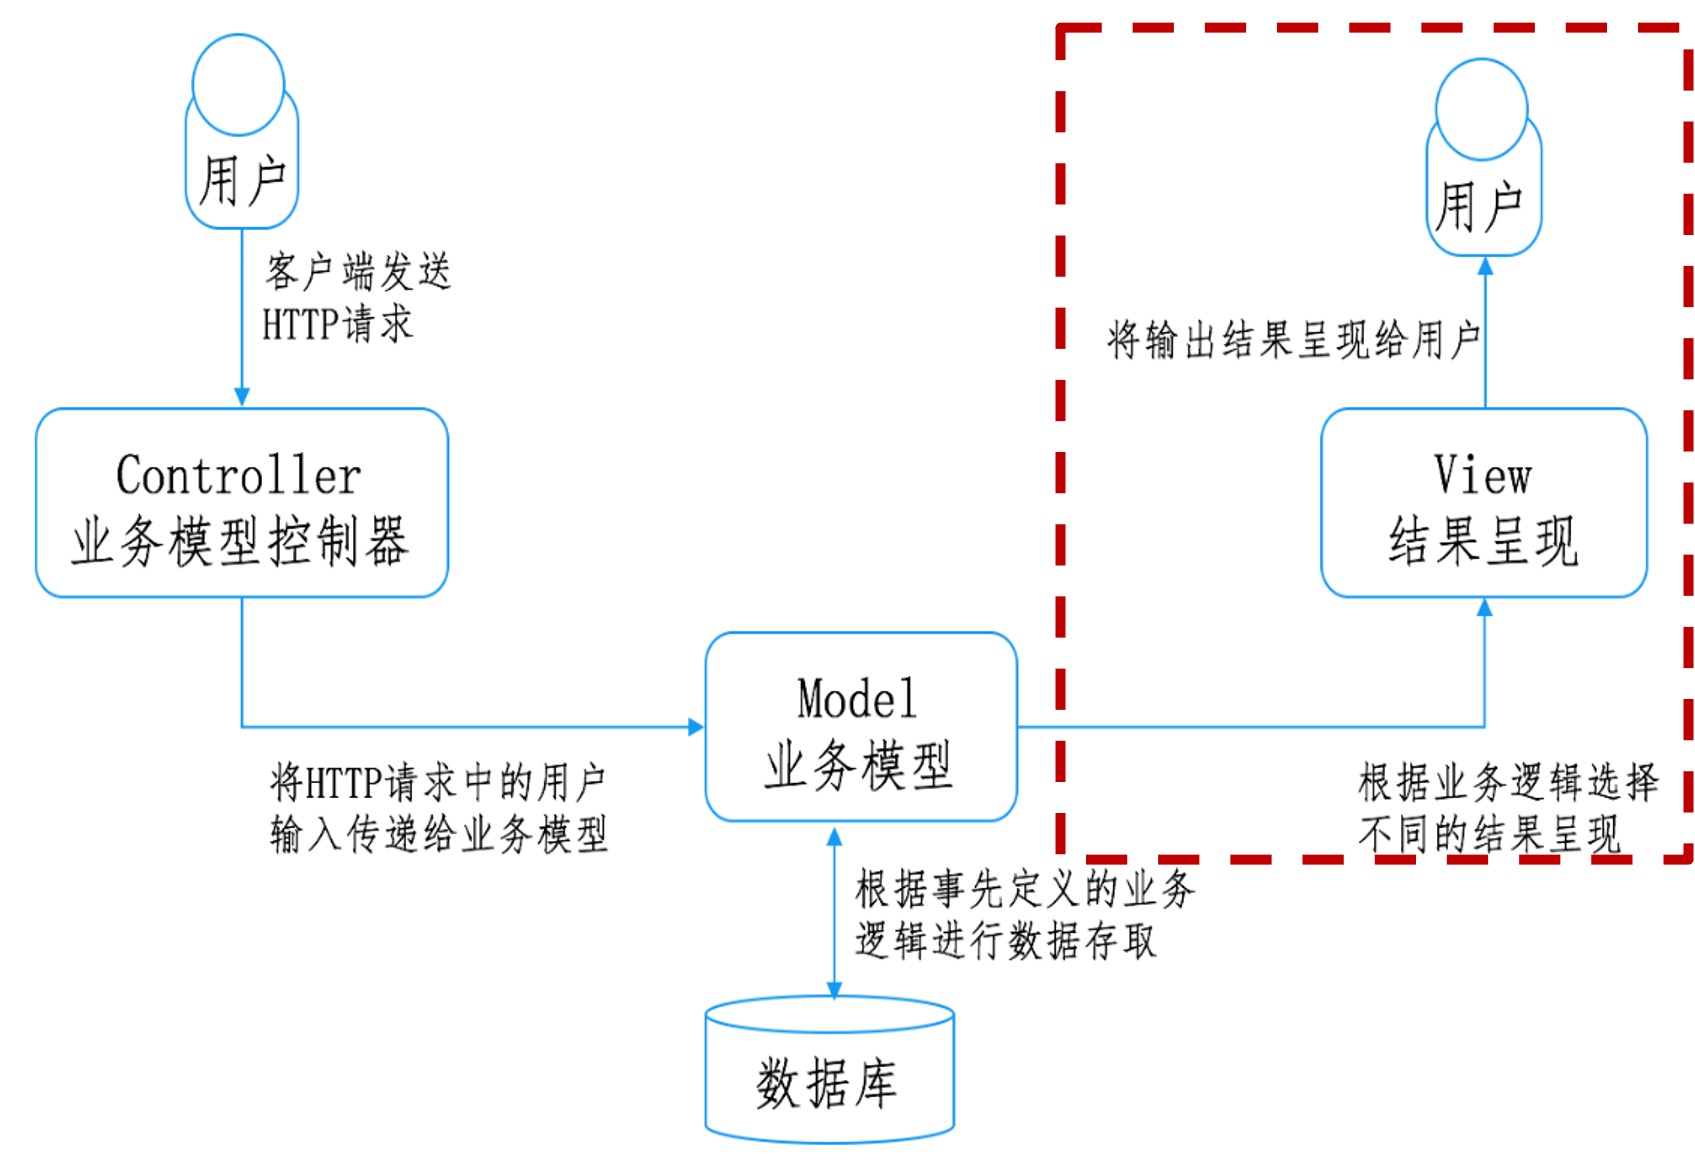
\includegraphics[width=\textwidth]{figure/fig-18.jpg}
\end{figure}

\end{frame}